\lab{Algorithms}{An Introduction to Parallel Programming using MPI}{Introduction to Parallel Programming}
\objective{Learn the basics of parallel computing on distributed memory machines using MPI for Python}
\objective{Learn how to write basic parallel algorithms such as the trapezoidal rule}
\label{lab:MPI_Intro}

\section*{Why Parallel Computing?}
Over the past few decades, vast increases in computational power have come through 
increased single processor performance, which have almost wholly been driven by smaller transistors.
However, these faster transistors generate more heat, which destabilizes circuits. 
The so-called ``heat wall'' refers to the physical limits of single processors to 
become faster because of the growing inability to sufficiently dissipate heat.

To get around this physical limitation, parallel computing was born.
It began, as with most things, in many different systems and styles, involving various systems. 
Some systems had shared memory between many processors and some systems had a separate 
program for each processor while others ran all the processors off the same base program.

Today, the most commonly used method for high performance computing is a single-program,
multiple-data system with message passing. 
Essentially, these supercomputers are made up of many, many normal computers, each with their own memory. 
These normal computers are all running the same program and are able to communicate with each other. Although they all run the same program file, each process takes a different execution path through the code, as a result of the interactions that message passing makes possible.

Note that the commands being executed by process \emph{a} are going to be different 
from process \emph{b}. Thus, we could actually write two separate computer programs 
in different files to accomplish this. 
However, the most common method today has become to write both processes in a single program, 
using conditionals and techniques from the Message Passing Interface to control which 
lines of execution get assigned to which process.

This is a very different architecture than ``normal'' computers, and it requires a 
different kind of software. You can't take a traditional program and expect it to 
magically run faster on a supercomputer; you have to completely design a new algorithm 
to take advantage of the unique opportunities parallel computing gives.

\section*{MPI: the Message Passing Interface}
At its most basic, the Message Passing Interface (MPI) provides functions for sending 
and receiving messages between different processes.

MPI was developed out of the need for standardization of programming parallel systems. 
It is different than other approaches in that MPI does not specify a particular language. 
Rather, MPI specifies a library of functions--the syntax and semantics of message passing routines--that can be called from other programming languages, 
such as Python and C. MPI provides a very powerful and very general way of expressing parallelism. 
It can be thought of as ``the assembly language of parallel computing,'' because of this 
generality and the detail that it forces the programmer to deal with
\footnote{Parallel Programming with MPI, by Peter S. Pacheco, p. 7}.
In spite of this apparent drawback, MPI is important because it was the first portable, 
universally available standard for programming parallel systems and is the \emph{de facto} standard. 
That is, MPI makes it possible for programmers to develop portable, parallel software libraries,
an extremely valuable contribution.
Until recently, one of the biggest problems in parallel computing was the lack of software. 
However, parallel software is growing faster thanks in large part to this standardization. 

\begin{problem}
Most modern personal computers now have multicore processors. 
In order to take advantage of the extra available computational power, a single program must be specially designed. 
Programs that are designed for these multicore processors are also ``parallel'' programs, typically written using POSIX threads or OpenMP.
MPI, on the other hand, is designed with a different kind of architecture in mind. 
How does the architecture of a system for which MPI is designed differ what POSIX threads or OpenMP is designed for? 
What is the difference between MPI and OpenMP or Pthreads?
\end{problem}

\section*{Why MPI for Python?}
In general, parallel programming is much more difficult and complex than in serial. 
Python is an excellent language for algorithm design and for solving problems that 
don't require maximum performance. 
This makes Python great for prototyping and writing small to medium sized parallel programs. 
This is especially useful in parallel computing, where the code becomes especially complex. 
However, Python is not designed specifically for high performance computing and its 
parallel capabilities are still somewhat underdeveloped, so in practice it is better 
to write production code in fast, compiled languages, such as C or Fortran.

We use a Python library, mpi4py, because it retains most of the functionality of 
C implementations of MPI, making it a good learning tool since it will be easy to 
translate these programs to C later. 
There are three main differences to keep in mind between mpi4py and MPI in C:
\begin{itemize}
    \item Python is array-based. C and Fortran are not.
    \item mpi4py is object oriented. MPI in C is not.
    \item mpi4py supports two methods of communication to implement each of the basic MPI commands. 
    They are the upper and lower case commands (e.g. \li{Bcast(...)} and \li{bcast(...)}). 
    The uppercase implementations use traditional MPI datatypes while the lower case use 
    Python's pickling method. Pickling offers extra convenience to using mpi4py, 
    but the traditional method is faster. In these labs, we will only use the uppercase functions.
\end{itemize}


\section*{Introduction to MPI}
As tradition has it, we will start with a Hello World program.
\lstinputlisting[style=fromfile]{hello.py}
Save this program as \texttt{hello.py} and execute it from the command line as follows:
\begin{lstlisting}[style=ShellInput]
$ mpirun -n 5 python hello.py
\end{lstlisting}
The program should output something like this:
\begin{lstlisting}[style=ShellOutput]
Hello world! I'm process number 3.
Hello world! I'm process number 2.
Hello world! I'm process number 0.
Hello world! I'm process number 4.
Hello world! I'm process number 1.
\end{lstlisting}
Notice that when you try this on your own, the lines will not necessarily print in order. 
This is because there will be five separate processes running autonomously, and we cannot 
know beforehand which one will execute its \li{print} statement first.

\begin{warn}
It is usually bad practice to perform I/O (e.g., call \li{print}) from any process 
besides the root process, though it can oftentimes be a useful tool for debugging.
\end{warn}

\section*{Execution}
How does this program work? As mentioned above, mpi4py programs are follow the single-program 
multiple-data paradigm, and therefore each process will run the same code a bit differently. 
When we execute 
\begin{lstlisting}[style=ShellInput]
$ mpirun -n 5 python hello.py
\end{lstlisting}
a number of things happen:

First, the mpirun program is launched. 
This is the program which starts MPI, a wrapper around whatever program you to pass into it. 
The ``-n 5'' option specifies the desired number of processes. 
In our case, 5 processes are run, with each one being an instance of the program ``python''. 
To each of the 5 instances of python, we pass the argument ``hello.py'' which is the name of our program's text file, 
located in the current directory. Each of the five instances of python then opens the 
\texttt{hello.py} file and runs the same program. 
The difference in each process's execution environment is that the processes are given 
different ranks in the communicator. Because of this, each process prints a different 
number when it executes.

MPI and Python combine to make wonderfully succinct source code. 
In the above program, the line \li{from mpi4py import MPI} loads the MPI module from the mpi4py package.
The line \li{COMM = MPI.COMM_WORLD} accesses a static communicator object, which represents a group of processes which can communicate with each other via MPI commands.

The next line, \li{RANK = COMM.Get_rank()}, is where things get interesting. 
A ``rank'' is the process's id within a communicator, and they are essential to learning 
about other processes. When the program mpirun is first executed, it creates a 
global communicator and stores it in the variable \li{MPI.COMM_WORLD}. 
One of the main purposes of this communicator is to give each of the five processes a 
unique identifier, or ``rank''. When each process calls \li{COMM.Get_rank()}, 
the communicator returns the rank of that process. 
\li{RANK} points to a local variable, which is unique for every calling process 
because each process has its own separate copy of local variables. 
This gives us a way to distinguish different processes while writing all of the source code 
for the five processes in a single file.

In more advanced MPI programs, you can create your own communicators, which means that 
any process can be part of more than one communicator at any given time. 
In this case, the process will likely have a different rank within each communicator.


Here is the syntax for \li{Get_size()} and \li{Get_rank()}, where \li{Comm} is a communicator object:
\begin{description}
\item[Comm.Get\_size()]
Returns the number of processes in the communicator. It will return the same number to every process.
Parameters:
\begin{description}
    \item[Return value] - the number of processes in the communicator
    \item[Return type] - integer
\end{description}
Example:
\lstinputlisting[style=FromFile]{Get_size_example.py}
\item[Comm.Get\_rank()]
Determines the rank of the calling process in the communicator.
Parameters:
\begin{description}
    \item[Return value] - rank of the calling process in the communicator
    \item[Return type] - integer
\end{description}
Example:
\lstinputlisting[style=FromFile]{Get_rank_example.py}
\end{description}

\begin{problem}
Write the ``Hello World'' program from above so that every process prints out its 
rank and the size of the communicator 
(for example, process 3 on a communicator of size 5 prints ``Hello World from process 3 out of 5!'').
\end{problem}

\section*{The Communicator}
A communicator is a logical unit that defines which processes are allowed to 
send and receive messages. In most of our programs we will only deal with the \li{MPI.COMM_WORLD} 
communicator, which contains all of the running processes. 
In more advanced MPI programs, you can create custom communicators to group only a small 
subset of the processes together. By organizing processes this way, MPI can 
physically rearrange which processes are assigned to which CPUs and optimize your 
program for speed. Note that within two different communicators, the same process 
will most likely have a different rank.

Note that one of the main differences between mpi4py and MPI in C or Fortran, 
besides being array-based, is that mpi4py is largely object oriented. 
Because of this, there are some minor changes between the mpi4py implementation of 
MPI and the official MPI specification.

For instance, the MPI Communicator in mpi4py is a Python class and MPI functions 
like \li{Get_size()} or \li{Get_rank()} are instance methods of the communicator class. 
Throughout these MPI labs, you will see functions like \li{Get_rank()} presented as 
\li{Comm.Get_rank()} where it is implied that \li{Comm} is a communicator object.

\section*{Separate Codes in One File}
When an MPI program is run, each process receives the same code. 
However, each process is assigned a different rank, allowing us to specify separate 
behaviors for each process. In the following code, all processes are given the same two numbers. 
However, though there is only one file, 3 processes are given completely different instructions 
for what to do with them. Process 0 sums them, process 1 multiplies them, 
and process 2 takes the maximum of them:
\lstinputlisting[style=FromFile]{separateCode.py}

\begin{problem}
Write a program in which the the processes with an even rank print ``Hello'' and 
process with an odd rank print ``Goodbye.'' 
Print the process number along with the ``Hello'' or ``Goodbye'' 
(for example, ``Goodbye from process 3'').
\end{problem}

\begin{problem}
Sometimes the program you write can only run correctly if it has a certain number of processes. 
Although you typically want to avoid writing these kinds of programs, sometimes it is 
inconvenient or unavoidable. Write a program that runs only if it has 5 processes. 
Upon failure, the root node should print ``Error: This program must run with 5 processes'' 
and upon success the root node should print ``Success!'' To exit, call the function 
\li{COMM.Abort()}.
\end{problem}

As was mentioned the simplest message passing involves two processes: a sender and a receiver. We will use these methods to parallelize the Trapezoidal Rule.

\section*{Simple Message Passing}
Let us begin by demonstrating a program designed for two processes. One will draw a random number and then send it to the other. We will do this using the routines \li{Comm.Send} and \li{Comm.Recv} (short for ``receive''):

\lstinputlisting[style=FromFile]{passValue.py}

To illustrate simple message passing, we have one process choose a random number and then pass it to the other. Inside the recieving process, we have it print out the value of the variable \li{num_buffer} \emph{before} it calls \li{Recv} to prove that it really is recieving the variable through the message passing interface.

Here is the syntax for \li{Send} and \li{Recv}, where \li{Comm} is a communicator object:

\begin{description}
\item[Comm.Send(buf, dest=0, tag=0)]
Performs a basic send. This send is a point-to-point communication. It sends information from exactly one process to exactly one other process.
Parameters:
\begin{description}
\item[buf (array-like)] – data to send.
    
% TODO expand here- must be numpy array (as a pointer) and won't work with strings

\item[dest (integer)] – rank of destination
\item[tag (integer)] – message tag
\end{description}
Example:
\lstinputlisting[style=FromFile]{Send_example.py}
\item[Comm.Recv(buf, source=0, tag=0, Status status=None)]
Basic point-to-point receive of data.
Parameters:
\begin{description}
\item[buf (array-like)] – initial address of receive buffer (choose receipt location)
\item[source (integer)] – rank of source
\item[tag (integer)] – message tag
\item[status (Status)] – status of object
\end{description}
Example:
See example for Send()
\end{description}

\begin{info}
\li{Send} and \li{Recv} are referred to as \emph{blocking} functions. That is, if a process calls \li{Recv}, it will sit idle until it has received a message from a corresponding \li{Send} before it will proceeed. (However, the process that calls \li{Comm.Send} will \emph{not} necessarily block until the message is recieved- it depends on the implementation) There are corresponding \emph{non-blocking} functions \li{Isend} and \li{Irecv} (The \emph{I} stands for immediate). In essence, \li{Irecv} will return immediately. If a process calls \li{Irecv} and doesn't find a message ready to be picked up, it will indicate to the system that it is expecting a message, proceed beyond the \li{Irecv} to do other useful work, and then check back later to see if the message has arrived. This can be used to dramatically improve performance.
\end{info}

% TODO ASK is Send blocking in C? It isn't in python... I added in a note here

\begin{info}
When calling \li{Comm.Recv}, you can allow the calling process to accept a message from any process that happend to be sending to the receiving process. This is done by setting source to a predefined MPI constant, \li{source=ANY_SOURCE} (note that you would first need to import this with from \li{mpi4py.MPI import ANY_SOURCE} or use the syntax \li{source=MPI.ANY_SOURCE}).
\end{info}


\begin{problem}
Write a Python script \texttt{passVector.py} (adapted from \texttt{passValue.py}) that passes an $n$ by $1$ vector of random values from one process to the other. Write it so that the user passes the value of $n$ in as a command-line argument (similar to the code developed later in this lab for the trapezoidal rule).
\end{problem}

\begin{problem}
Try modifying some of the parameters in \li{Send} and \li{Recv} in the code from the previous exercise (\li{dest}, \li{source}, and \li{tag}).  What happens to the program? Does it hang or crash? What do you suppose the \li{tag} parameter does?
\end{problem}
% TODO delete this one?

\begin{problem}
Write a Python script \texttt{passCircular.py} (again adapted from \texttt{passValue.py}). This time, write the program so that each process with rank $i$ sends a random value to the process with rank $i+1$ in the global communicator. The process with the highest rank will send its random value to the root process. Notice that we are communicating in a ring. For communication, only use \li{Send} and \li{Recv}. The program should work for any number of processes. (Hint: Remember that \li{Send} and \li{Recv} are blocking functions. Does the order in which \li{Send} and \li{Recv} are called matter?)
% TODO \li{} for referencing file?
\end{problem}

\section*{The Trapezoidal Rule}
Now that we understand basic communication in MPI, we will proceed by parallelizing our first algorithm--numerical integration using the ``trapezoidal rule.'' Early on in most calculus classes, students learn to estimate integrals using the trapezoidal rule. A range to be integrated is divided into many vertical slivers, and each sliver is approximated with a trapezoid. The area of each trapezoid is computed, and then all their areas are added together.

% LaTeX to display the trapezoidal rule:
\begin{eqnarray*}%{rcl}
\textrm{Area} 
&\approx&
\sum_{i=0}^{n-1}\frac{[f(a+i \Delta x)+f(a + (i+1) \Delta x)]}{2}\cdot\Delta x \\
&=&
\left[-\frac{f(a)+f(b)}{2}+\sum_{i=0}^{n}f(a+i\Delta x)\right]\cdot\Delta x
\end{eqnarray*}
where $\Delta x=(b-a)/n$.

% Trapezoid rule picture:
\begin{figure}[h]
\centering
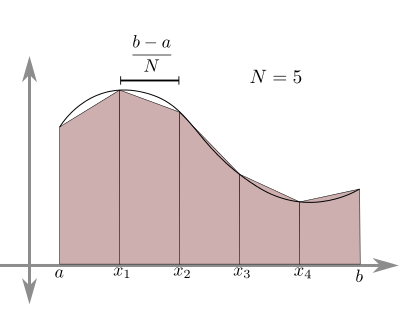
\includegraphics[width=.5\textwidth]{TrapezoidRule.png}
\caption{The trapezoid rule in action. TODO get a copyright-kosher version.}
\label{fig:trapezoidal_rule}
\end{figure}
% I took this template for icluding images from the data structures lab

In Python, a simple serial formulation of the trapezoidal rule would be as follows:

\lstinputlisting[style=FromFile]{trapSerial.py}

A moment of thought should convince the reader that this algorithm reflects the formula given above. 

\section*{Parallelizing the Trapezoidal Rule}
The first and most important step in parallelizing an algorithm is determining which computations are independent. With the trapezoidal rule, it's easy to see that the area of each trapezoid can be calculated independently, so dividing the data at the trapezoid level seems natural.

Currently, the algorithm divides up the interval into $n$ subintervals. To parallelize this process, we will distribute these $n$ subintervals to the available processes:

\lstinputlisting[style=FromFile]{trapParallel_1.py}

In this parallel approach, the original interval is split such that each process gets an equal-sized subinterval to integrate. After integrating, each process sends its result to the root node, which sums up the results and displays them. Although this is fairly straightforward, there are two important things to note:

First, notice how the trapezoids are divided among the processes: The processors each individually calculate the specifics of which subinterval they will be integrating. We could have written the algorithm such that process 0 divides up the work for the other processors and tells them each what their ranges are. However, this would introduce an unnecessary bottleneck: all of the other processes would be idling while waiting for their assignment to arrive from the root process. By having each process calculate its own range, we gain a large speedup.

Second, notice how the results are summed. We know how many results we should be receiving, so the root process simply accepts the messages in the order that they arrive. This is achieved using the tag \li{MPI.ANY_SOURCE} in the \li{COMM.Recv} method. In following labs we will learn about even more effective ways to gather the results of many different processes' computations.
% todo link to lab where we learn gather (next lab). Talk about the speed up we gained here? but in this case there is no speedup...

% MPI has two mechanisms specifically designed to partition the message space: tags and communicators. The tag parameter is there in the case that two messages with the same size and datatype are sent to the same process. In that case, the program would not necessarily be able to tell apart the data. So the programmer can attach different tags that he or she defines to the sent data to keep them straight.
% TODO find somewhere else for this paragraph to fit in maybe? Maybe as the answer to that problem from the intro that asks what tags do?

At this point, you should test the code for yourself. Save the code in a file named \texttt{trapParallel\_1.py} and try running it from the command line using the following input: 
\begin{lstlisting}[style=ShellInput]
$ mpirun -n 4 python trapParallel_1.py 0.0 1.0 10000
\end{lstlisting}
The output should appear like this:
\begin{lstlisting}[style=ShellOutput]
With 10000 trapezoids, our estimate of the integral of x^2 from 0.0 to 1.0 is:
    0.333333335
\end{lstlisting}
We have successfully parallelized our first algorithm!


\section*{Load Balancing}
Although we have parallelized the trapezoidal rule, our algorithm is still rather naive. Notice that if the number of processes does not evenly divide the number of trapezoids, the code will break down. Try running the trapezoid program with n = 10007 trapezoids:
\begin{lstlisting}[style=ShellInput]
$ mpirun -n 4 python trapParallel_1.py 0.0 1.0 10007
\end{lstlisting}
This will produce the following:
\begin{lstlisting}[style=ShellOutput]
With 10007 trapezoids, our estimate of the integral of x^2 from 0.0 to 1.0 is:
    0.333233404949
\end{lstlisting}

We know that the estimate of the integral should improve as $n$ grows larger, but this estimate is much worse. This happened because \li{local_n}, the number of trapezoids that each processor calculates, must be an integer. To solve this problem, we could require that the user always choose a value of $n$ that is divisible by the number of processors. However, good parallel code should let the user worry as little as possible about the parallelization and should function exactly as the serial version does. Thus, we should improve the code to let it handle the case where $n$ is not divisible by the number of processes.

One way to solve this problem would be to designate one process to handle the leftover trapezoids that; i.e. give each process \li{int(n/SIZE)} trapezoids and assign the remaining \li{n \% SIZE} trapezoids to the last process as well. Thus, the \li{local_n} of each process would be an integer. However, this method can be incredibly inefficient: What if we ran the program with $100$ processes and $n=1099$ trapezoids? Then each process would have \li{int(1099/100) = 10} trapezoids to calculate... except for the last process, which would have \li{10 + 1099 \% 100 = 109} trapezoids!

\emph{A parallel program can only be as fast as its slowest process.} We call this principle \emph{load balancing}. In this case, one process has to do over ten times as much work as the other processes! The other processes will end up waiting idle until the last one finishes. Ignoring communication costs and other overhead, this program could be nearly 10 times faster if we divided up the work more evenly. The important concept to remember is that any time a process is idling, we are losing efficiency.

In the case of the trapezoidal rule, load-balancing the code means two things. First, between any two processes, the number of trapezoids given to each must differ by at most $1$. Second, each process should estimate the area of a contiguous group of trapezoids. Although estimating an integral is not a very time-consuming operation, by estimating over contiguous groups of trapezoids we are minimizing the amount of duplicate work the processes have to do, which is good practice.

\begin{problem}
Implement the \emph{load-balancing} fix to the code \texttt{trapParallel\_1.py}. The program should be able to take in any number of trapezoids $n$ for any number of processes and the trapezoids should be divided among the processes evenly, differing by at most one between any two processes. Each process should independently calculate which section of trapezoids it should calculate.

For example, if the program is run with 5 processes and 12 trapezoids, processes 0 should calculate the first 3 trapezoids, process 1 should calculate the next 3 trapezoids, process 2 should calculate the next 2 trapezoids, process 3 should calculate the next 2 trapezoids, and process 4 should calculate the last 2 trapezoids.
\end{problem}
